\chapter*{Apêndice 3: Controlador de versão}
\label{ap3:github}

Neste Apêndice serão apresentados os passos necessários para a criação do repositório utilizado no sistema de controle de versão, junto com a instalação da ferramenta utilizada para trabalhar com este controlador de versão e sua configuração.

Para criar um repositório no GitHub (ferramenta de controle de versão) utilizado neste trabalho, deve-se acessar a  \textit{url} http://github.com, por meio de um navegador de internet e clicar no botão \textit{"Sign In"}, caso possua conta, caso contrário clique no botão \textit{"Sign up"} e crie sua conta. A Figura~\ref{fig:ap3:pagina_inicial_github} apresenta a página inicial do GitHub.

\captionsetup[figure]{list=no}
\begin{figure}[h!]
	\centerline{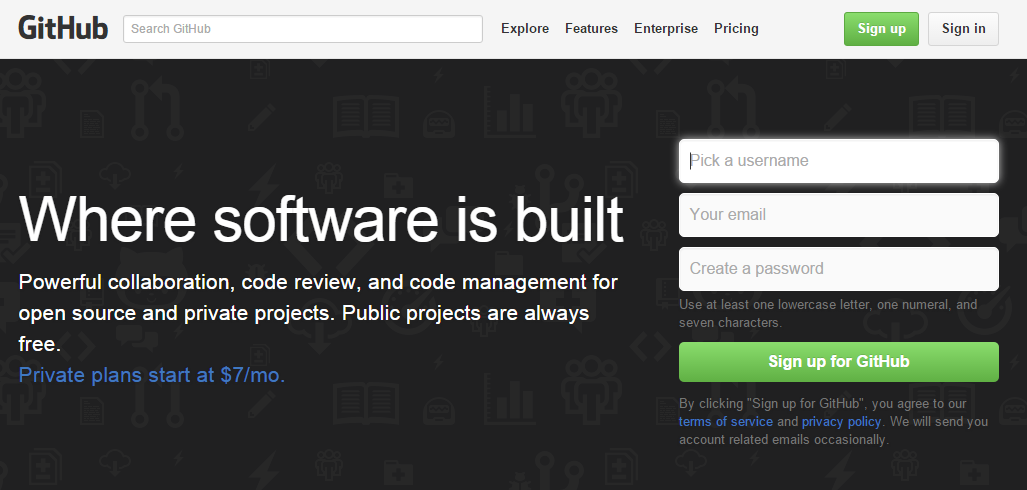
\includegraphics[scale=0.5]{./imagens/apendices/pagina-inicial-github.png}}
	\caption[Página inicial do GitHub.]
	{Página inicial do GitHub. \textbf{Fonte:} Elaborado pelos autores.}
	\label{fig:ap3:pagina_inicial_github}
\end{figure}

Para prosseguir com o processo de criação do repositório (com a conta já criada), deve-se clicar no botão \textit{"Sign In"} e realizar o \textit{login}. Após a conclusão desses passos a página inicial, contendo a lista de repositórios do usuário será apresentada conforme a Figura~\ref{fig:ap3:pagina_home_github} apresenta.

\newpage
\captionsetup[figure]{list=no}
\begin{figure}[h!]
	\centerline{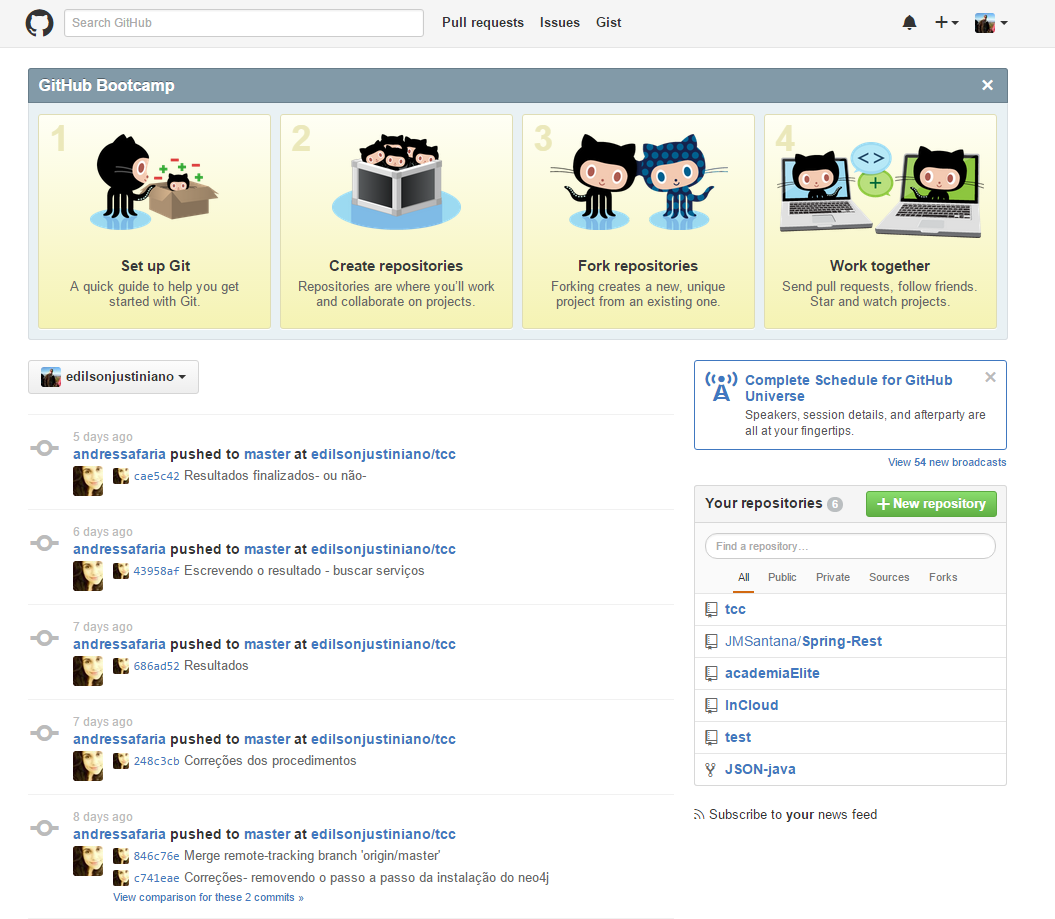
\includegraphics[scale=0.5]{./imagens/apendices/pagina-home-github.png}}
	\caption[Página com a lista de repositórios do usuário no GitHub.]
	{Página com a lista de repositórios do usuário no GitHub. \textbf{Fonte:} Elaborado pelos autores.}
	\label{fig:ap3:pagina_home_github}
\end{figure}


Na página inicial deve-se clicar no botão \textit{"+ New Repository"} para que a página de criação do novo repositório seja apresentada conforme a Figura~\ref{fig:ap3:pagina_criacao_repository_github} apresenta.
\newpage
\captionsetup[figure]{list=no}
\begin{figure}[h!]
	\centerline{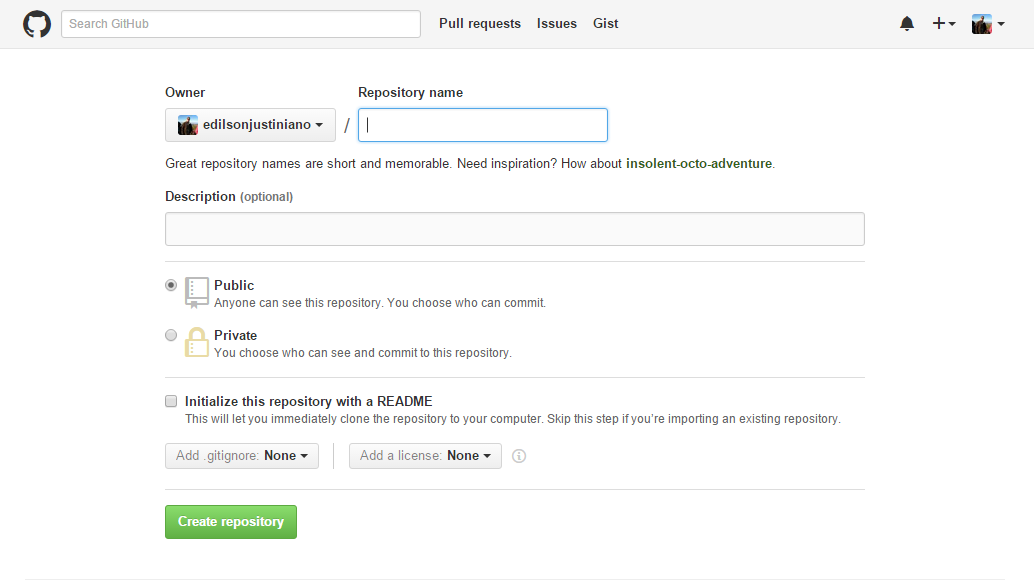
\includegraphics[scale=0.5]{./imagens/apendices/pagina-criacao-repositorio-github.png}}
	\caption[Página de criação de repositório no GitHub.]
	{Página de criação de repositório no GitHub. \textbf{Fonte:} Elaborado pelos autores.}
	\label{fig:ap3:pagina_criacao_repository_github}
\end{figure}

Nessa página deve-se informar os dados referentes ao repositório e, após preencher o formulário clique no botão \textit{"Create repository"}, a fim de concluir o processo de criação do repositório no GitHub.

Após criado o repositório, foi necessário adicionar os autores deste trabalho como colaboradores para que ambos pudessem modificar arquivos. Para fazer esta configuração é necessário clicar no menu \textit{"Settings"} da página inicial do repositório conforme apresenta a Figura~\ref{fig:ap3:pagina_inicial_repositororio_github}.

\newpage
\captionsetup[figure]{list=no}
\begin{figure}[h!]
	\centerline{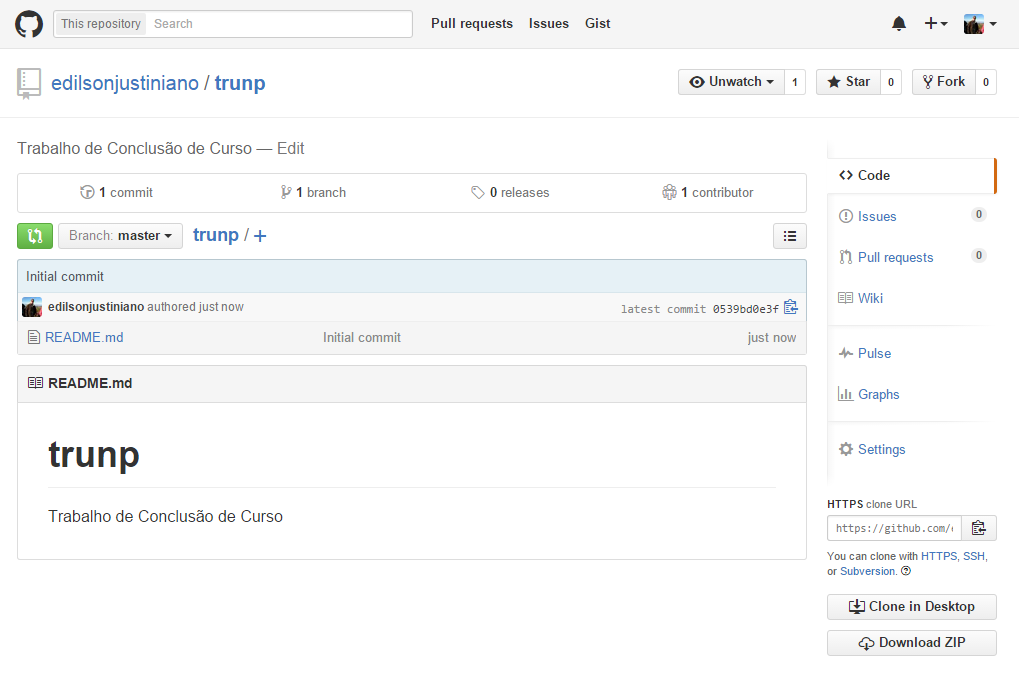
\includegraphics[scale=0.5]{./imagens/apendices/pagina-inicial-repositorio-github.png}}
	\caption[Página do repositório no GitHub.]
	{Página do repositório no GitHub. \textbf{Fonte:} Elaborado pelos autores.}
	\label{fig:ap3:pagina_inicial_repositororio_github}
\end{figure}

Após clicar no menu \textit{"Settings"} é necessário navegar até a opção \textit{"Collaborators"} e informar o email ou o nome de usuário do colaborador conforme apresenta a Figura~\ref{fig:ap3:pagina_adicionar_colaborador_repositorio_github}.

\captionsetup[figure]{list=no}
\begin{figure}[h!]
	\centerline{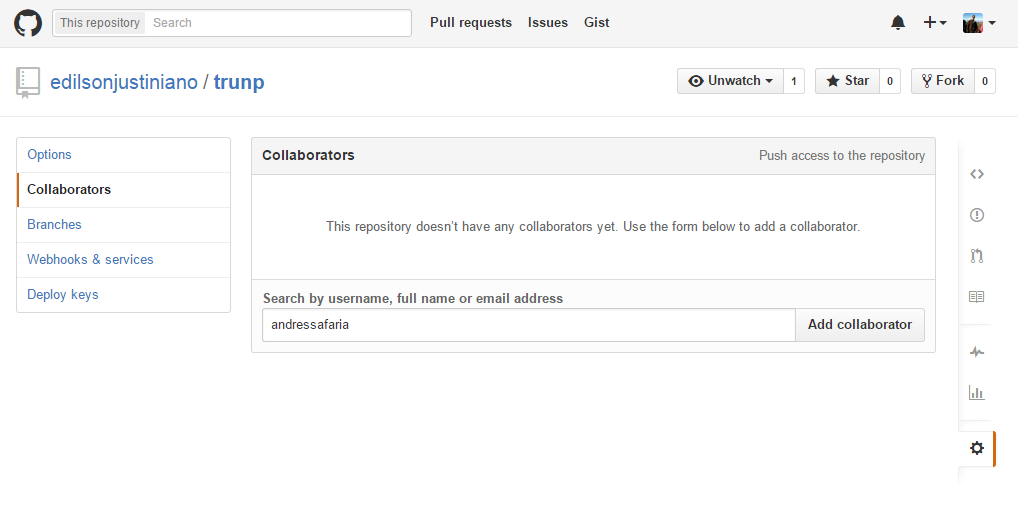
\includegraphics[scale=0.5]{./imagens/apendices/pagina-adicionar-colaborador-ao-repositorio.png}}
	\caption[Página para adicionar um contribuidor ao repositório no GitHub.]
	{Página para adicionar um contribuidor ao repositório no GitHub. \textbf{Fonte:} Elaborado pelos autores.}
	\label{fig:ap3:pagina_adicionar_colaborador_repositorio_github}
\end{figure}

Após informar o dado do usuário e clicar no botão \textit{"Add collaborator"} o repositório estará pronto para ser utilizado. Para facilitar o manuseio de arquivos e suas respectivas versões, neste controlador de versão foi utlizada a ferramenta gráfica disponibilizada pelo GitHub a fim de facilitar a utilização deste sistema de controle de versão. Para realizar o download desta ferramenta, acesse a \textit{url} https://desktop.github.com por meio de um navegador de internet e clique no botão de download como apresenta a Figura~\ref{fig:ap3:pagina_download_github_para_windows}.

\captionsetup[figure]{list=no}
\begin{figure}[h!]
	\centerline{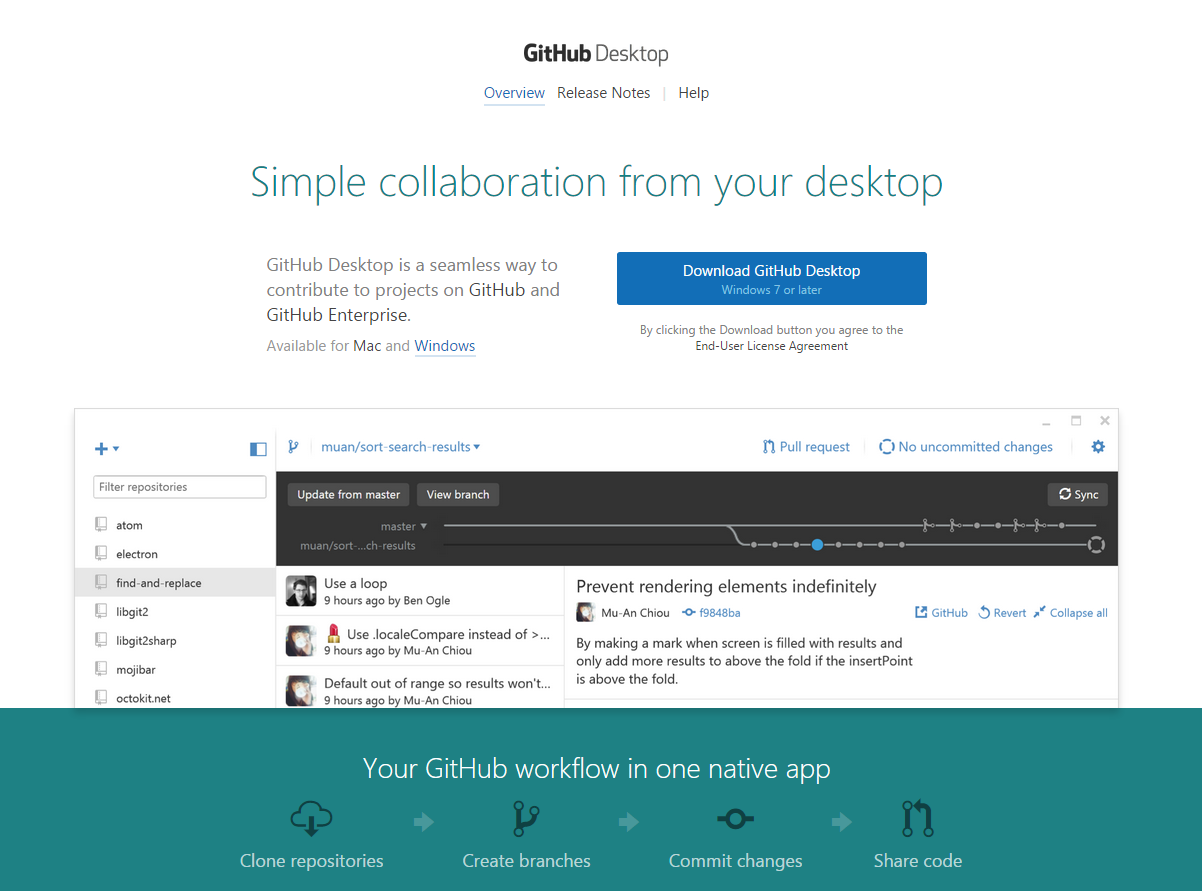
\includegraphics[scale=0.4]{./imagens/apendices/pagina-download-github.png}}
	\caption[Página de \textit{download} da ferramenta para gerenciamento de repositórios do GitHub.]
	{Página de \textit{download} da ferramenta para gerenciamento de repositórios do GitHub. \textbf{Fonte:} Elaborado pelos autores.}
	\label{fig:ap3:pagina_download_github_para_windows}
\end{figure}

Após realizar o download, deve-se executar o arquivo obtido por meio do processo de \textit{download} anteriormente mencionado. Após executá-lo, o processo de instalação da ferramenta irá iniciar, como apresenta a Figura~\ref{fig:ap3:instalacao_github_para_windows}.

\captionsetup[figure]{list=no}
\begin{figure}[h!]
	\centerline{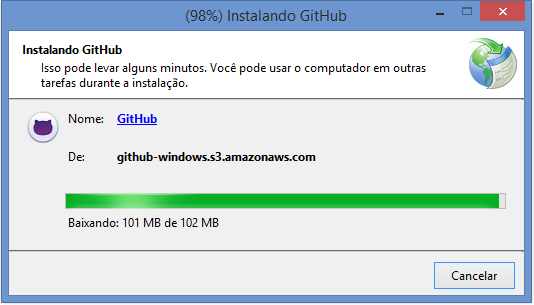
\includegraphics[scale=0.5]{./imagens/apendices/instalacao-github-step1.png}}
	\caption[Instalação da ferramenta para gerenciamento de repositórios do GitHub.]
	{Instalação da ferramenta para gerenciamento de repositórios do GitHub. \textbf{Fonte:} Elaborado pelos autores.}
	\label{fig:ap3:instalacao_github_para_windows}
\end{figure}

Após concluir a instalação da ferramenta execute-a para configurar o repositório local no computador de trabalho. Com a aplicação em execução clique no botão "+" e em seguida, no menu \textit{"Clone"}, após esses passos localize o repositório desejado e clique em \textit{"Clone Repository"} como apresenta a Figura~\ref{fig:ap3:clonar_repositorio_github}.

\newpage
\captionsetup[figure]{list=no}
\begin{figure}[h!]
	\centerline{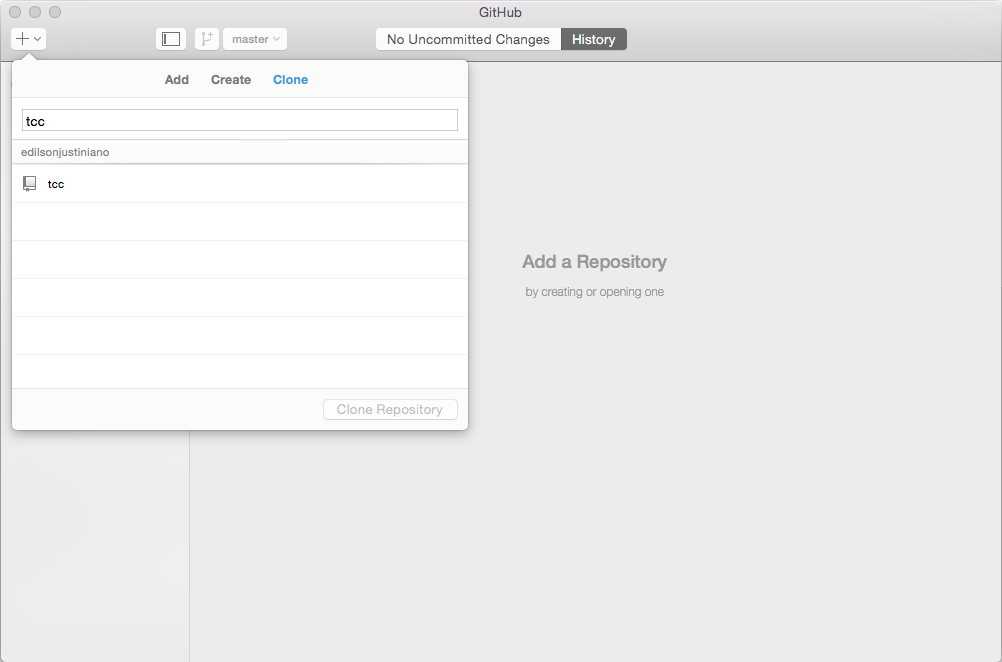
\includegraphics[scale=0.4]{./imagens/apendices/clonar-repositorio-github.png}}
	\caption[Processo para clonar repositório do GitHub.]
	{Processo para clonar repositório do GitHub. \textbf{Fonte:} Elaborado pelos autores.}
	\label{fig:ap3:clonar_repositorio_github}
\end{figure}

Após a realização dos passos descritos neste apêndice o repositório no GitHub estará totalmente configurado.